% ===================================================================================================
\chapter{Molecular Dynamics Simulations}
% ===================================================================================================

% ---------------------------------------------------------------------------------------------------
\section{Molecular Dynamics in General}
% ---------------------------------------------------------------------------------------------------
Molecular dynamics (MD) as a simulation method originates from the 1950s and is, therefore, one of the oldest tools used in computational physics and materials research \cite{alder1957phase}.
On a fundamental level, MD consists of solving many-body problems iteratively to determine the forces acting on individual particles. 
These calculations, too complex to have any analytical solutions, are performed using numerical methods and allow us to relatively accurately simulate the dynamic evolution of (semi-)classical systems of particles. 

A typical MD algorithm follows the pattern described in fig. \ref{MD-schema}. 
The simulation is initiated by giving each atom, $i=1,...,N$, an initial position $\mathbf{r}_i^{(0)}$ and random velocity $\mathbf{v}_i^{(0)}$, consistent with the desired net temperature of the system. 
The positions and velocities, $\mathbf{r}_i$ and $\mathbf{v}_i$, are then updated by solving Newton's equations of motion
\begin{align}
\mathbf{F}_i(\mathbf{r}_i,t) = m_i\frac{d^2\mathbf{r}_i}{dt^2} = m_i\mathbf{a}_i(t) = -\nabla_{r_i}V(\mathbf{r}_i)
\end{align}
where $m_i$ is the mass of atom i, positioned at $\mathbf{r}_i$. 
The forces $\mathbf{F}_i$ are determined from the interatomic potential $V(\mathbf{r}_i)$ and can be used to calculate the acceleration of each particle. 
The new positions and velocities are then simply evaluated as functions of the acceleration and the simulation time step $\Delta t$. 
The simulation then proceeds through repeated evaluations of the equations of motion, updating the system in increments of $\Delta t$ time units. 
In order to avoid catastrophic errors in the conservation of energy, the time step must be shorter than the inverse vibrational frequency of any process in the system, typically around 1 fs for many materials in equilibrium. \cite{choe2000determination}

% [Neighbour lists & force cutoff]
In its purest form, MD requires us to perform $O(N^2)$ force evaluations, with $N$ being the number simulated of particles. 
In a typical simulation, however, the particles only interact with a limited number of neighbours, and most long-range interactions can be safely disregarded. 
A common way of doing this is by declaring a cutoff radius for the force calculations, with only particles within this radius from particle $i$ taken into account when evaluating $\mathbf{F}_i(\mathbf{r}_i,t)$. 
The use of a force cutoff theoretically reduces the scaling of the algorithm down to $O(N)$. \cite{verlet1967computer}

% [Periodic boundaries] 
Despite the use of a force cutoff, most real-world materials are still far too large to be simulated accurately.
For instance, a typical metal has a number density of around $5\cdot 10^{22}$ atoms/cm$^3$, meaning that simulating even just a $100\times 100 \times 100$ nm$^3$ block of metal, generally considered to be the arbitrary lower limit of bulk materials, would require us to keep track of $5\cdot 10^7$ atoms.
A standard way of 'cheating' is through the use of \textit{periodic boundary conditions} (PBCs). 
PBCs imply that particles exiting the region of space confined by the simulation cell borders re-appear on the opposite side, as visualized in fig. (\ref{Fig:pbcs}). 
Since also interatomic forces are allowed to interact over cell borders, we effectively have the cell surrounded by infinitely many copies of itself.

\begin{figure}[!ht]
\center
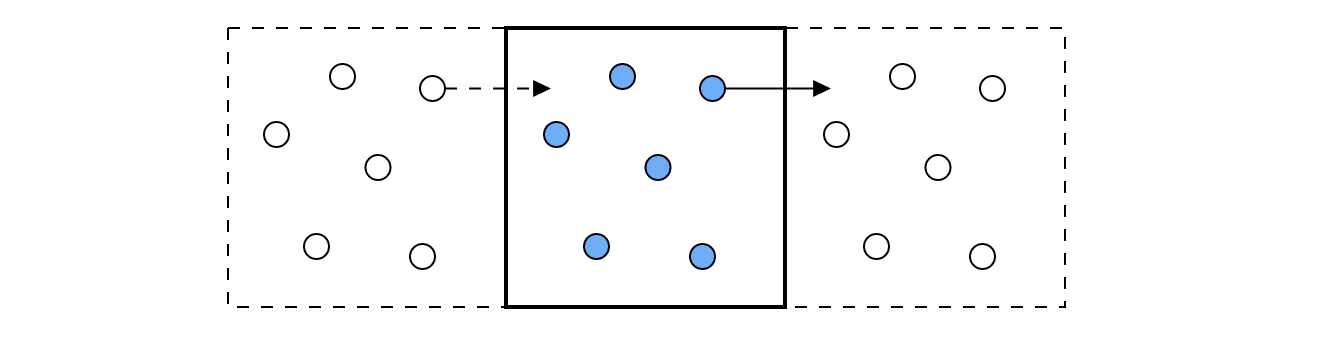
\includegraphics[width=0.75\linewidth]{pbc.png}
\caption{A visualization of periodic boundary conditions in a 2D simulation cell. The cells with dashed lines represent virtual copies}
\label{Fig:pbcs}
\end{figure}

With a perfect lattice, a simulation cell with periodic boundary conditions accurately emulates a bulk material. 
With various defects introduced, we, however, have to make sure that the cell is large enough for the created strain field not to overlap with itself, possibly affecting the results detrimentally.

% [Thermostats, barostats]
Real systems are seldom isolated and instead exchange at least energy with their surroundings in a number of ways. 
In order to sample a non-isolated thermodynamic ensemble, we need to control the temperature of our simulation manually. 
Temperature of an atomic system is defines as
\begin{align}
T(t) = \frac{1}{k_{\text{B}}N_f}\sum_{i}\left[ m_iv_{i,x}^2(t) + m_iv_{i,y}^2(t) + m_iv_{i,z}^2(t)\right]
\end{align}
where $N_f$ is the number of degrees of freedom and $v_{i}$ is the velocity of atom $i$. 
It is, therefore, straightforward to see why we can control the temperature by scaling atomic velocities.
A common and relatively simple way of doing this is called the \textit{Berendsen thermostat} and defined as
\begin{align}
\frac{dT}{dt} = \frac{T_0-T}{\tau}
\end{align}
where $T_0$ is the target temperature and $\tau$ a time constant \cite{berendsen1984molecular}. 
Despite its high efficiency, the Berendsen thermostat is not producing a correct canonical ensemble and is prone to causing various unphysical artefacts.

The \textit{Nos\'{e}-Hoover thermostat}, on the other hand, accurately samples the canonical ensamble \cite{nose1984unified}. 
Being a so-called \textit{extended system method}, the Nos\'{e}-Hoover thermostat makes use of a virtual particle reservoir, effectively acting as a heat bath. 
Since this requires equations of motions to be evaluated both for the actual particles and the virtual reservoir, the gained physical accuracy comes at a higher computational cost.

% --------------- MD schematic ------------------------------------------------------------------------------------
\begin{figure}
\begin{center}
% Define block styles
\tikzset{
decision/.style = {diamond, draw, fill=green!40, 
    text width=4.5em, text badly centered, node distance=3cm, inner sep=0pt},
block/.style = {rectangle, draw, fill=cyan!30, 
    text width=20em, text centered, rounded corners, minimum height=2em},
cloud/.style = {draw, ellipse,fill=red!20, node distance=3cm,
    minimum height=2em}
    }

\begingroup  % compress equations
\medmuskip=2mu
\thinmuskip=1mu
\thickmuskip=2mu
\begin{tikzpicture}
\matrix (m)[matrix of nodes, column  sep=1.5cm,row  sep=5mm, align=center, nodes={rectangle,draw, anchor=center} ]{
    |[block]| {Set initial conditions $\mathbf{r}_i(t_0)$ and $\mathbf{v}_i(t_0)$, set a timestep $dt$ and reset $\mathbf{a}=0$, $_0t=0$}              &  \\
    %|[block]| {\textit{Estimation step:}\\ Estimate new atom positions; \\
    %  Move atoms: $\mathbf{r}_i^{(e)} = \mathbf{r}_i^{(j)} + \mathbf{v}^{(j)}dt + \mathbf{a}\frac{1}{2}dt^2 + ...$\\
    %  Update velocities: $\mathbf{v}^{(e)}=\mathbf{v}^{(f)}+\mathbf{a}dt + ...$}              &  \\
   |[block]| {Calculate $\mathbf{F}_i = -\mathbf{\nabla} V(\mathbf{r}_i)$ and $\mathbf{a}_i=\mathbf{F}_i/m_i$}              &  \\
   |[block]| {Adjust atom positions based on the new $\mathbf{a}_i$;\\
     Move atoms: $\mathbf{r}_i(t_{n+1}) = \mathbf{r}_i(t_n) + f(\mathbf{a}_i,\Delta t)$\\
      Update velocities: $\mathbf{v}(t_{n+1})=\mathbf{v}(t_n)+g(\mathbf{a}_i,\Delta t)$}              &  \\
   |[block]| {Apply boundary conditions, thermostats and barostats as needed}              &  \\
   |[block]| {Calculate and output physical quantities of interest}              &  \\
   |[block]| {$t_{n+1} = t_n+\Delta t$}              &  \\
   |[decision]| {End condition reached?}              &  \\
   |[block]| {Collect data and quit}              &  \\
};
\path [>=latex,->] (m-1-1) edge (m-2-1);
\path [>=latex,->] (m-2-1) edge (m-3-1);
\path [>=latex,->] (m-3-1) edge (m-4-1);
\path [>=latex,->] (m-4-1) edge (m-5-1);
\path [>=latex,->] (m-5-1) edge (m-6-1);
\path [>=latex,->] (m-6-1) edge (m-7-1);
%\path [>=latex,->] (m-7-1) edge (m-8-1);
\draw [>=latex,->] (m-7-1.west) -- node[above] {no} ++(-4,0cm) |- (m-2-1.west);
\draw [>=latex,->] (m-7-1.south) -- node[right] {yes}(m-8-1);
\end{tikzpicture}
\endgroup
\caption{A flowchart representation of a typical Molecular Dynamics simulation. Above, $f$ and $g$ refer to two different functions of the timestep and the acceleration. In the most simple case these would be $f(\mathbf{a}_i,\Delta t) = \mathbf{v}_i\Delta t + \mathbf{a}_i\Delta t^2$ and $g(\mathbf{a}_i,\Delta t) = \mathbf{a}_i\Delta t$, respectively.} 
\label{MD-schema}
\end{center}
\end{figure}
%------------------------------------------------------------------------------------------------------------------


\subsection{Interatomic potentials}

In an MD simulation, potential energies of simulated particles are calculated using so-called \textit{interatomic potentials} - mathematical functions designed to approximately emulate the interactions between atoms. 
These potentials are usually based upon the Born-Oppenheimer model, i.e. that the electrons of all atoms are permanently in the ground state and that all interactions depend purely on the interatomic distance \cite{born1927quantentheorie}. 
In general terms, the potential energy of an atomistic system can be written as
\begin{align}
V_{tot} = \sum_i^N V_1(\mathbf{r}_i) + \sum_{i,j}^N V_2(\mathbf{r}_i, \mathbf{r}_j) +  \sum_{i,j,k}^N V_3(\mathbf{r}_i, \mathbf{r}_j, \mathbf{r}_k) + ...
\label{V_tot-ekv}
\end{align}
where $N$ is the number of atoms in the system and $V_1$, $V_2$ and $V_3$ respectively are one, two and three body terms \cite{potentialsTheory}.

The indices $i$, $j$ and $k$ iterate through the atom positions in three spatial dimensions and can be restricted to $i < j$ and $j < k$ for symmetric interactions such as those encountered in periodic, monoelemental systems. 
The first term of eq. (\ref{V_tot-ekv}) can be discarded for systems not affected by an external field, an we are thus left with
\begin{align}
V_{tot} = \sum_i \sum_{j>i} V_2(\mathbf{r}_i, \mathbf{r}_j) + \sum_i \sum_{j>i} \sum_{k > j} V_3(\mathbf{r}_i, \mathbf{r}_j, \mathbf{r}_k) + ...
\end{align}
Potentials employing terms of a higher order than two are referred to as many-body potentials, while those using only the two first terms are pair potentials.

The atomic structure of metals allows them to be described particularly well using the so-called \textit{Embedded Atom Method} (EAM) formalism, giving the potential energy in the form
\begin{align}
V_{tot} = \sum_i^N F_i\, \bigg( \sum_j \rho\, (\mathbf{r}_{ij}) \bigg) + \frac{1}{2} \sum^N_{ij} V_2 (\mathbf{r}_{ij})
\end{align}
where  $F_i$ is a function of the summed electron density $\rho (\mathbf{r}_{ij})$ and $\mathbf{r}_{ij}$ denotes the distance $| \mathbf{r}_i - \mathbf{r}_j |$ between the $i$th and $j$th atoms. \cite{EAMmodel,dudarevEAMpotential}. 

For covalently bonded materials, it is often more accurate to use a \textit{Bond Order Potential} (BOP), generally presented as
\begin{align}
V_{ij}(r_{ij}) =bV_{ijk}V_{\rm attractive}(r_{ij}) V_ {\rm repulsive}
\end{align}
Examples of BOPs are potentials of Tersoff, Brenner and Finnis-Sinclair type. \cite{tersoff1988new, brenner1990empirical, finnis1984simple} Both BOP and EAM potentials have the functional shape of a typical pair-potential, but act as many-body potentials due to many-body interactions embedded into the pair-terms.

\section{Parallel Algorithms}
Doubling the side length of a cubical atomic system increases the number of atoms by a factor of eight. 
Correspondingly, the number of necessary force calculations increases by a factor of  8 to 64, depending on the use of neighbour lists.
Since we at any given time only store a minimal amount of vector data per atom, MD simulations are generally not very memory intensive.
Computationally, however, they are indeed expensive due to the large number of force evaluations performed every time step.

Interestingly, the nature of MD simulations makes them inherently parallel, allowing the forces for all atoms to be calculated simultaneously. 
This fact can be exploited by dividing the computational load across multiple processing units. 
Parallellisation on $P$ processors can be performed using three principal algorithms; \textit{atom-}, \textit{spatial-} and \textit{force-decompositon}. 
\cite{fincham1987parallel}

The atom-decompositon algorithm includes appointing $N/P$ atoms to each processor and requires \textit{all-to-all} communication of forces between processors and therefore it scales as $O(N)$, independently of $P$. 
The force-decomposition algorithm, on the other hand, divides the cell into three-dimensional boxes, with atoms being re-appointed to the corresponding processor each time they enter a new box. 
This method limits the communication required to only neighbouring processors, giving a theoretical scaling of $O(N/P)$ for largely parallel simulations.
The spatial-decomposition algorithm, finally, involves appointing force calculation loops to separate processors.
This method is fairly non-trivial to grasp and achieves at best a scaling of $O(N/\sqrt{P})$, lagging behind the spatial-decomposition algorithm in performance. \cite{fincham1987parallel,lammpsMD}

% ---------------------------------------------------------------------------------------------------
% \section{Analysis of the Results}
% --------------------------------------------------------------------------------------------------- 

